\documentclass[11pt]{article}

\usepackage[margin=1in]{geometry}
\usepackage{booktabs}
\usepackage{amsmath}
\usepackage{graphicx}
% Figures are generated by src/figures.py into preprint/. Referencing
% them rather than duplicating keeps one copy under version control;
% both directories live in the same repository.
\graphicspath{{../preprint/}}
\usepackage{xcolor}
\usepackage{microtype}
\usepackage{caption}
\usepackage{array}
\usepackage[hidelinks]{hyperref}

\newcommand{\cfg}[1]{\texttt{#1}}
\newcommand{\best}[1]{\textbf{#1}}
\captionsetup{font=small}

\title{\textbf{Quantizing ESM-2 for Protein Language Modelling:\\
A Measurement Study on Speed, Memory, and Accuracy}}
\author{Qing Shao\\[2pt]
Department of Chemical and Materials Engineering, University of Kentucky\\[2pt]
\emph{Benchmarking report --- ESM2-3B on NVIDIA H200 and A100}}
\date{7 August 2026}

\begin{document}
\maketitle

\begin{abstract}
\noindent
We benchmark six numerical precision configurations for ESM-2 protein language
models across three axes --- throughput, memory footprint, and predictive
accuracy --- on two workloads with sharply different characteristics: bulk
embedding extraction and deep mutational scanning (DMS) variant-effect scoring.
Accuracy is evaluated on the complete ProteinGym substitution benchmark ---
201 assays, 2.41M variants --- at \textbf{three model scales spanning 650M to
15B parameters}, with a paired bootstrap clustered on protein. Three findings
follow. First, \textbf{benchmark averages conceal the failure that decides
deployability}: no configuration shifts mean correlation by more than $0.007$ at
any scale, yet INT8 dynamic quantization --- indistinguishable from fp32 on that
mean at 3B ($p = 0.34$) --- takes a single assay from $\rho = 0.591$ to $0.223$.
Second, \textbf{fidelity against fp32 bounds risk but cannot rank quality}: over
3015 assay/configuration pairs it predicts the \emph{magnitude} of ground-truth
change ($r = 0.56$--$0.81$) but not its \emph{direction}, and INT4 weight-only
quantization is significantly harmful at 650M, significantly \emph{beneficial}
at 3B, and null at 15B --- a reversal with no monotone trend to extrapolate.
Third, \textbf{the configuration ranking is itself scale-dependent}: FP8 dynamic
quantization runs at $0.50\times$ bf16 DMS throughput at 650M and $1.01\times$
at 15B while halving memory, so the workload conflict that dominates at small scale
dissolves at large scale. We also report four measurement artifacts encountered
during this study, three of which inverted the result they were meant to
measure.
\end{abstract}

\section{Introduction}

Quantization is usually presented as a straightforward trade: reduce numerical
precision, gain speed and memory, lose a little accuracy. This framing is
inherited from large autoregressive language models, where it is broadly
correct. We set out to test whether it transfers to ESM-2, a family of protein
language models, and found that essentially every part of it requires
qualification.

ESM-2 is a BERT-style bidirectional \emph{encoder}. It performs a single forward
pass with no KV cache and no autoregressive decode. This places it in a
\textbf{compute-bound} regime rather than the memory-bandwidth-bound regime that
governs LLM inference at batch size 1. The distinction is not academic: the
dominant open-source quantization toolchains (GPTQ, AWQ, bitsandbytes NF4, GGUF)
are all \emph{weight-only}. They store INT4/INT8 weights and dequantize to bf16
immediately before an ordinary bf16 matrix multiply. When the bottleneck is
memory bandwidth, this is a large win. When the bottleneck is arithmetic, as it
is here, it adds work to an already-saturated kernel.

This report addresses three questions:

\begin{enumerate}
  \item What do the available quantization configurations actually cost and
        deliver on the three axes of speed, memory, and accuracy?
  \item Does the answer depend on the workload? (It does, and the two workloads
        we study prefer opposite configurations.)
  \item Do the fidelity metrics conventionally used to validate quantization
        predict real-world predictive accuracy? (Only partially, and in a way
        that matters.)
\end{enumerate}

\section{Experimental Design}

\subsection{Configurations}

Six configurations were evaluated, all applied via \texttt{torchao} to the
encoder \texttt{Linear} layers only:

\begin{table}[htb]
\centering
\caption{Quantization configurations. Weight-only variants target memory; the
dynamic (W8A8) variants also quantize activations and can therefore use
low-precision tensor cores for the matrix multiply itself.}
\small
\begin{tabular}{llp{7.4cm}}
\toprule
Configuration & Class & Description \\
\midrule
\cfg{fp32}     & baseline    & Reference for all fidelity measurements. \\
\cfg{bf16}     & baseline    & The practical production default. \\
\cfg{int8\_wo} & weight-only & INT8 weights, bf16 compute. Memory-oriented. \\
\cfg{int4\_wo} & weight-only & INT4 weights, bf16 compute. Smallest footprint. \\
\cfg{int8\_dyn}& W8A8        & INT8 weights \emph{and} dynamically quantized
                               activations; uses INT8 tensor cores. \\
\cfg{fp8\_dyn} & W8A8        & FP8 (E4M3) weights and activations. Requires
                               compute capability $\geq 8.9$; H200 only. \\
\bottomrule
\end{tabular}
\end{table}

\subsection{Workloads}

\textbf{Bulk embedding extraction.} Large length-bucketed batches under a token
budget, measured in residues per second. This is the compute-bound regime.

\textbf{DMS variant-effect scoring.} The standard ESM masked-marginals protocol:
for each mutated position, mask it and record
$\log p(\text{mut}) - \log p(\text{wt})$ from the resulting distribution. Cost
scales with the \emph{number of mutated positions}, not with the number of
variants, and the masked batch is narrow. This is the latency-bound regime.

Two optimizations were applied to the DMS path before benchmarking, both of
which are absent from typical reference implementations: only positions
carrying a variant are masked, and the masked copies are batched rather than
run one at a time.

\subsection{Metrics}

Three fidelity metrics were recorded, deliberately ordered by sensitivity:

\begin{enumerate}
  \item \textbf{Embedding cosine similarity} (mean-pooled, excluding special
        tokens and padding). Forgiving: error averages out along the sequence.
  \item \textbf{Logit KL divergence}, per residue. Moderately sensitive.
  \item \textbf{DMS Spearman $\rho$ against fp32.} Most sensitive, because the
        score is a \emph{difference of two near-equal log-probabilities}, so
        quantization noise does not cancel and is amplified relative to signal.
\end{enumerate}

All three are drift-from-fp32 measures. They quantify how far a configuration
moves the answer, not whether it moves toward or away from the truth. To measure
the latter, we added a fourth metric requiring real experimental data:
\textbf{Spearman $\rho$ against wet-lab DMS measurements}, from ProteinGym.

\subsection{Real assay data}

Three ProteinGym substitution assays were selected to span the sequence-length
range, since peak memory during masked-marginals scoring grows with $L$:

\begin{table}[htb]
\centering
\caption{ProteinGym assays used. All 19{,}557 single-substitution variants had
their stated wild-type residue verified against the reference \texttt{target\_seq}
before use; all matched. This check is load-bearing --- an off-by-one in
position indexing does not raise an error, it silently scores the wrong
positions and yields a plausible-looking correlation.}
\small
\begin{tabular}{lrrrl}
\toprule
Assay & $L$ & Singles & Masked positions & Coverage \\
\midrule
\texttt{IF1\_ECOLI\_Kelsic\_2016}     &  72 &  1{,}367 &  72 & 100\% \\
\texttt{BLAT\_ECOLX\_Stiffler\_2015}  & 286 &  4{,}996 & 263 &  92\% \\
\texttt{HSP82\_YEAST\_Flynn\_2019}    & 709 & 13{,}194 & 707 & 100\% \\
\bottomrule
\end{tabular}
\end{table}

\subsection{Full benchmark data}

The three-assay analysis is superseded by a run over the complete ProteinGym
substitution benchmark. All 217 assays were extracted from the
\texttt{ProteinGym\_v1} parquet release and every one passed wild-type
validation across 2{,}465{,}767 variants. The 201 assays fitting ESM-2's
1022-residue context were scored: 2{,}413{,}913 variants over 40{,}775 masked
positions, spanning $L = 37$ to $934$ and five function categories.

The masked-position count, not the variant count, sets the cost: masked-marginals
scoring performs one forward pass per mutated position, so 2.41M variants are
nearly free on top of 40{,}775 forwards.

An earlier three-assay path combined per-assay CSVs from the \texttt{v0.1}
release with wild-type sequences from the \texttt{v1.0} reference file. The two
agree on the 85 assays present in both and diverge elsewhere, including renames.
That is acceptable for three hand-picked assays and unsafe at benchmark scale;
the \texttt{v1} parquet carries \texttt{target\_seq} inline, so scores and
wild-type sequences come from a single release.

\subsection{Comparability to published benchmark numbers}
\label{sec:comparability}

Two choices make our absolute correlations not directly comparable to a
published ESM-2 ProteinGym figure.

\textbf{The aggregation convention matters more than any effect we measure.}
An unweighted mean over assays, a mean of per-protein means, and a mean of
per-category means are all defensible and give different answers spanning
$0.019$ --- roughly three times the largest quantization effect here.

\begin{table}[htb]
\centering
\caption{fp32 mean Spearman under four aggregation conventions. The flat mean we
report is the most favourable of the four. The \emph{differences between
configurations} are stable across all four: signs identical, magnitudes within
$\sim$$0.001$, the sole exception being \cfg{int8\_dyn} under category weighting,
which was not significant under any convention.}
\label{tab:agg}
\small
\begin{tabular}{lrrr}
\toprule
Aggregation & ESM2-650M & ESM2-3B & ESM2-15B \\
\midrule
Flat mean over 201 assays (this report) & 0.4459 & 0.4398 & 0.4323 \\
Mean of per-protein means               & 0.4403 & 0.4377 & 0.4321 \\
Mean of per-category means              & 0.4297 & 0.4209 & 0.4152 \\
Post-stratified to the full 217         & 0.4406 & 0.4355 & 0.4290 \\
\bottomrule
\end{tabular}
\end{table}

\textbf{The 16 excluded assays are not a random sample.} They exceed ESM-2's
context ($L = 1154$--$3423$) and are 2.1\% of benchmark variants, but 50\% are
low-MSA-depth against 13.9\% retained, and none are stability assays against
32.8\% retained. Low-MSA-depth assays score far worse, so the exclusion inflates
any unweighted mean --- post-stratifying to the full-217 composition costs about
$0.004$ at 3B. It also \emph{understates} \cfg{int4\_wo}'s harm at 650M, which
moves from $-0.0064$ to $-0.0068$ under post-stratification.

Run \texttt{python src/analyze\_scales.py} to reproduce all four conventions.

\subsection{Statistical treatment}

Ground-truth correlations are compared using a \textbf{paired bootstrap} (2000
resamples). Both the candidate configuration and the fp32 reference are scored
on the \emph{same} resample at each iteration, so shared noise cancels and the
residual is attributable to the configuration. The pairing is not a refinement:
for \cfg{int4\_wo} the paired interval is $8.4\times$ narrower than the unpaired
one, because per-assay $\rho$ spans $0.0$--$0.9$ while the configuration effect is
of order $0.006$. Unpaired, every configuration reads as noise.

The \emph{resampling unit} differs by scale of claim. For a single assay the
unit is the variant, which establishes that a shift is not an artifact of the
variant set. For the full benchmark the unit is the assay, since the claim
becomes one about assays in general. Because the 201 assays cover only 173
distinct proteins, benchmark-level intervals use a \textbf{cluster bootstrap
over proteins}: whole proteins are drawn and all their assays retained, so
correlated replicates cannot count as independent evidence. Clustered and
unclustered intervals agreed to the fourth decimal, which is reported as a
measured result rather than assumed.

Intervals are percentile bootstrap. They were checked against a normal
approximation ($\bar{d} \pm 1.96\,\mathrm{SE}$) and agree to four decimals on
every configuration, confirming the underlying distribution is near-symmetric
and the percentile method is not distorting the interval. The procedure was
validated on synthetic data with a known answer: a negligible perturbation was
correctly classified as noise, a genuine improvement as real.

\subsection{Measurement repeatability}
\label{sec:repeat}

Every difference reported here is at $10^{-4}$ resolution or finer, and the tail
statistic is a \emph{maximum} over 201 assays --- a quantity any noise inflates,
since the maximum of many noisy draws is large even when every true effect is
zero. Neither is interpretable without knowing what the pipeline does when
nothing changes, so we measured it rather than assuming determinism.

The complete benchmark was re-run for all six configurations at 650M and for
\cfg{bf16} and \cfg{int8\_dyn} at 3B, as separate jobs on different physical
GPUs. Across 8 model/configuration replicates and $19{,}311{,}304$ per-variant score
comparisons, \textbf{every score is identical} at the $10^{-6}$ precision to
which scores are stored. Per-assay Spearman is unchanged to five decimals,
benchmark means to six, and the largest per-assay $|\Delta\rho|$ between two
runs of the same configuration is $0.00000$.

So the null for the tail statistic is exactly zero --- there is no run-to-run
variability for a maximum to select from, and a worst-assay $\Delta\rho$ of
$-0.369$ is entirely attributable to the configuration. Differences of $0.0002$
are properties of the configuration rather than of the run. And the headline
collapse reproduces exactly: \texttt{UBR5\_HUMAN\_Tsuboyama\_2023\_1I2T} gives
$\rho = 0.2226$ under \cfg{int8\_dyn} at 3B in both runs.

Caveats. Determinism removes run-to-run variance and nothing else; the
assay-sampling uncertainty the bootstrap quantifies is untouched, and a
reproducible $0.0002$ is still negligible. Both runs used H200 GPUs and one
software stack, so determinism across GPU architectures or torch/torchao
versions is not established. Scores are stored rounded to six decimals, so
``identical'' means identical to $10^{-6}$ --- three orders below the smallest
effect discussed.

Reproduce with \texttt{python src/analyze\_repeat.py}.

\subsection{Hardware and software environment}

\begin{table}[htb]
\centering
\small
\begin{tabular}{ll}
\toprule
Component & Detail \\
\midrule
GPU (primary)  & NVIDIA H200, 143\,GB, sm\_90 (FP8 tensor cores) \\
GPU (secondary)& NVIDIA A100, 80\,GB, sm\_80 (no FP8) \\
Driver         & 550.54.14 \\
PyTorch        & 2.6.0+cu124 \\
Attention      & SDPA \\
Compile mode   & \texttt{max-autotune-no-cudagraphs} \\
\bottomrule
\end{tabular}
\end{table}

The cluster runs CentOS 7.6 with glibc 2.17 on every node, including the H200
nodes, which forced several choices. PyTorch moved to \texttt{manylinux\_2\_28}
at version 2.7, making \textbf{2.6.0 the newest installable release}.
\texttt{bitsandbytes} GPU wheels require a newer glibc, so only the CPU-only
0.42.0 installs and its NF4 path is unavailable --- 4-bit quantization therefore
goes through \texttt{torchao}. The system GCC (4.8.5) cannot build Triton's
helper module, so \texttt{torch.compile} fails until \texttt{CC}/\texttt{CXX}
are pointed at GCC 12.1.0. Finally, \texttt{\$HOME} and \texttt{/project} are at
quota, and the Triton, Inductor, HuggingFace, and pip caches all default there;
all were relocated to \texttt{/scratch}. \texttt{torchao} nonetheless works
because its INT8/FP8 paths dispatch to \texttt{torch.\_int\_mm} and
\texttt{torch.\_scaled\_mm}, which live inside PyTorch and support sm\_90.

\section{Results}

Sections~\ref{sec:compile}--\ref{sec:pilotscale} establish the speed, memory and
fidelity behaviour of each configuration on the two workloads, taking ground
truth from three hand-picked assays --- enough to show that an effect exists on
a particular assay, not enough to generalise from it.
Section~\ref{sec:full} repeats the accuracy measurement on the complete
201-assay benchmark at three model scales and overturns two conclusions the
three-assay pilot supported; each retraction is stated where the original claim
was made.

\subsection{Compile mode determines whether W8A8 is viable at all}
\label{sec:compile}

The single most consequential configuration choice is not the quantization
scheme but the \texttt{torch.compile} mode. Measured on a single ESM2-3B-shaped
feed-forward block, $2560 \to 10240 \to 2560$, at batch $32 \times 512$ on an
A100:

\begin{table}[htb]
\centering
\caption{Only \texttt{max-autotune} allows Inductor to autotune the INT8 Triton
matmuls, which is where the entire W8A8 benefit resides.}
\small
\begin{tabular}{lr}
\toprule
Variant & Time (ms) \\
\midrule
bf16 eager                                   & 7.91 \\
bf16 compiled                                & 7.91 \\
\cfg{int8\_dyn} eager                        & 33.35 \\
\cfg{int8\_dyn} compiled, \texttt{dynamic=True} & 11.73 \\
\cfg{int8\_dyn} compiled, default mode       & 11.48 \\
\cfg{int8\_dyn} \texttt{mode="max-autotune"} & \best{5.43} \\
\bottomrule
\end{tabular}
\end{table}

Measured in eager mode, W8A8 appears $4.2\times$ \emph{slower} than bf16 and
would be discarded. Measured under \texttt{max-autotune} it is $1.46\times$
faster. \texttt{dynamic=True} was avoided because it emits shape-generic kernels
that surrender most of the gain; static shapes are kept manageable by padding to
a fixed multiple of 128. \texttt{torch.\_dynamo.explain} confirms \textbf{zero
graph breaks} for both bf16 and \cfg{int8\_dyn}, establishing this as a
kernel-selection effect rather than a Dynamo fallback.

\subsection{Bulk embedding extraction}

\begin{table}[htb]
\centering
\caption{ESM2-3B, H200, compiled with \texttt{max-autotune-no-cudagraphs}, SDPA
attention, 64 sequences of length 512--1024 under a 16{,}384-token budget.
Reproduced across five independent jobs: bf16 mean 56{,}789 residues/s, range
55{,}941--57{,}422 ($\pm 1.3\%$); fp32 mean 6{,}752, range 6{,}687--6{,}814. The
\cfg{int8\_dyn\_asym} row is from the fifth job at identical settings, whose
bf16 (57{,}377) and \cfg{int8\_dyn} (60{,}023) fall inside those ranges.}
\small
\begin{tabular}{lrrrrrrr}
\toprule
Config & Weights & Peak & Residues/s & vs bf16 & Emb.\ cos & Logit KL & DMS $\rho_{\text{fp32}}$ \\
       & (GB)    & (GB) &            &         &           &          & \\
\midrule
\cfg{fp32} (ref)  & 10.72 & 25.37 &  6{,}750 & 0.12$\times$ & ---      & ---      & --- \\
\cfg{bf16}        &  5.29 & 12.63 & 57{,}057 & 1.00$\times$ & 0.999949 & 1.17e--04 & 0.9998 \\
\cfg{int8\_wo}    &  2.66 &  8.48 & 54{,}816 & 0.96$\times$ & 0.999959 & 1.05e--04 & 0.9998 \\
\cfg{int8\_dyn}   &  2.65 & \best{7.07} & 59{,}996 & 1.05$\times$ & 0.989592 & 1.40e--02 & 0.9928 \\
\cfg{int8\_dyn\_asym} & 2.65 &  7.26 & 51{,}383 & 0.90$\times$ & 0.999469 & 1.41e--03 & 0.9972 \\
\cfg{fp8\_dyn}    &  2.65 &  7.24 & \best{65{,}376} & \best{1.15$\times$} & 0.999920 & 4.60e--04 & 0.9988 \\
\cfg{int4\_wo}    & \best{1.61} &  7.69 &  3{,}813 & 0.07$\times$ & 0.998904 & 1.89e--03 & 0.9975 \\
\bottomrule
\end{tabular}
\end{table}

Three observations. First, the \textbf{fp32 $\to$ bf16 step is worth
$8.4\times$} --- larger than everything quantization adds on top of it, and the
single biggest lever available. Second, \cfg{fp8\_dyn} dominates
\cfg{int8\_dyn}: it is faster ($1.15\times$ vs $1.05\times$) \emph{and}
dramatically more accurate (embedding cosine 0.999920 vs 0.989592; logit KL
$4.6\times10^{-4}$ vs $1.4\times10^{-2}$), surrendering only 0.17\,GB of peak
memory. FP8's E4M3 format has far greater dynamic range than INT8 at the same
bit width, which matters because transformer activations contain outliers.
Third, \cfg{int4\_wo} is a trap for inference: $0.07\times$ throughput and
\emph{worse} peak memory (7.69\,GB) than \cfg{fp8\_dyn} (7.24\,GB) despite 40\%
smaller weights, because the dequantization path allocates transient buffers.
Its value lies elsewhere, as a QLoRA base.

Separately, length-bucketed batching reduced padding waste from 25.0\% (naive
fixed-size batching) to \textbf{0.0\%}. This is free and costs no accuracy ---
a larger effect than several of the quantization differences in the table.

\subsection{DMS scoring: the opposite conclusion}

\begin{table}[htb]
\centering
\caption{DMS scoring throughput, ESM2-3B, uncompiled. bf16 wins at every problem
size; quantization is pure overhead in this regime.}
\small
\begin{tabular}{lrrr}
\toprule
Config & \multicolumn{3}{c}{Variants/s} \\
\cmidrule(lr){2-4}
       & IF1 ($L{=}72$) & BLAT ($L{=}286$) & HSP82 ($L{=}709$) \\
\midrule
\cfg{bf16}      & \best{6{,}979} & \best{3{,}573} & \best{1{,}357} \\
\cfg{int8\_wo}  & 4{,}830 & 2{,}511 & 1{,}066 \\
\cfg{fp8\_dyn}  & 1{,}813 & 1{,}796 & 1{,}103 \\
\cfg{fp32}      & 1{,}460 &   447 &   187 \\
\cfg{int8\_dyn} &   410 &   382 &   299 \\
\cfg{int4\_wo}  & 1{,}045 &   282 &   112 \\
\bottomrule
\end{tabular}
\end{table}

bf16 is fastest at every assay size, and \cfg{int8\_dyn} --- the second-fastest
configuration for bulk extraction --- is up to $17\times$ slower here. The
masked batch (n\_positions $\times$ $L$) is too small to contain a matrix
multiply large enough for low precision to pay for its quantize/dequantize
overhead.

Notably, \cfg{fp8\_dyn} closes on bf16 as the assay grows: $0.26\times$,
$0.50\times$, $0.81\times$ of bf16 throughput at $L = 72, 286, 709$
respectively. Its overhead is fixed per call while real work scales, so at
$L=709$ it costs 20\% throughput for 43\% less memory --- a defensible trade
that is indefensible at $L=72$.

\subsection{Memory during DMS scoring}

\begin{table}[htb]
\centering
\caption{Peak device memory during DMS scoring. Weights account for
approximately 90\% of peak even at $L=709$ (bf16: 5.29\,GB weights against
0.59\,GB activations).}
\small
\begin{tabular}{lrrrr}
\toprule
Config & Weights (GB) & Peak $L{=}72$ & Peak $L{=}286$ & Peak $L{=}709$ \\
\midrule
\cfg{fp32}      & 10.72 & 10.87 & 11.19 & 11.85 \\
\cfg{bf16}      &  5.29 &  5.38 &  5.55 &  5.88 \\
\cfg{int8\_wo}  &  2.66 &  2.77 &  2.92 &  3.25 \\
\cfg{int8\_dyn} &  2.65 &  2.87 &  2.91 &  3.36 \\
\cfg{fp8\_dyn}  &  2.65 &  2.76 &  2.96 &  3.35 \\
\cfg{int4\_wo}  & \best{1.61} & \best{1.70} & \best{1.87} & \best{2.20} \\
\bottomrule
\end{tabular}
\end{table}

This is the reverse of the bulk-extraction situation. Masked-marginals scoring
keeps the batch narrow, so the $O(L^2)$ attention term never dominates and
weights remain roughly 90\% of peak memory even at $L=709$. Quantization
therefore addresses almost all of DMS peak memory, and \cfg{int4\_wo} gives the
smallest footprint at every length --- $2.7\times$ below bf16.

\subsection{Ground-truth accuracy on ProteinGym}
\label{sec:gt}
\label{sec:gt}

\begin{table}[htb]
\centering
\caption{Spearman correlation against experimental measurements, ESM2-3B.
$\Delta$ is the change from fp32, with a 2000-sample paired bootstrap over
variants. ``Real'' indicates the 95\% confidence interval excludes zero.}
\small
\begin{tabular}{llrrrl}
\toprule
Assay & Config & $\rho_{\text{expt}}$ & $\Delta$ vs fp32 & 95\% CI of $\Delta$ & Verdict \\
\midrule
IF1        & \cfg{fp32}      & 0.5561 & (ref)    &                      &  \\
($n{=}1367$)& \cfg{bf16}      & 0.5543 & $-0.0018$ & $[-0.0027, -0.0009]$ & \textbf{real} \\
           & \cfg{int8\_wo}  & 0.5570 & $+0.0009$ & $[-0.0003, +0.0021]$ & noise \\
           & \cfg{int8\_dyn} & 0.5504 & $-0.0057$ & $[-0.0124, +0.0013]$ & noise \\
           & \cfg{fp8\_dyn}  & 0.5584 & $+0.0023$ & $[-0.0022, +0.0067]$ & noise \\
           & \cfg{int4\_wo}  & 0.5394 & $\mathbf{-0.0167}$ & $[-0.0263, -0.0074]$ & \textbf{real} \\
\midrule
BLAT       & \cfg{fp32}      & 0.5893 & (ref)    &                      &  \\
($n{=}4996$)& \cfg{bf16}      & 0.5896 & $+0.0003$ & $[-0.0003, +0.0009]$ & noise \\
           & \cfg{int8\_wo}  & 0.5913 & $+0.0019$ & $[+0.0011, +0.0029]$ & \textbf{real} \\
           & \cfg{int8\_dyn} & 0.6160 & $\mathbf{+0.0266}$ & $[+0.0219, +0.0315]$ & \textbf{real} \\
           & \cfg{fp8\_dyn}  & 0.6088 & $\mathbf{+0.0194}$ & $[+0.0161, +0.0229]$ & \textbf{real} \\
           & \cfg{int4\_wo}  & 0.6388 & $\mathbf{+0.0495}$ & $[+0.0433, +0.0561]$ & \textbf{real} \\
\midrule
HSP82      & \cfg{fp32}      & 0.2931 & (ref)    &                      &  \\
($n{=}13194$)& \cfg{bf16}    & 0.2933 & $+0.0002$ & $[-0.0002, +0.0005]$ & noise \\
           & \cfg{int8\_wo}  & 0.2933 & $+0.0002$ & $[-0.0002, +0.0007]$ & noise \\
           & \cfg{int8\_dyn} & 0.2937 & $+0.0006$ & $[-0.0020, +0.0028]$ & noise \\
           & \cfg{fp8\_dyn}  & 0.2944 & $+0.0012$ & $[-0.0003, +0.0027]$ & noise \\
           & \cfg{int4\_wo}  & 0.2904 & $-0.0027$ & $[-0.0057, +0.0002]$ & noise \\
\bottomrule
\end{tabular}
\end{table}

Two findings emerge, and the second qualifies the first.

\paragraph{Quantization does not systematically degrade variant-effect
accuracy.} Of the 15 assay/configuration pairs, 11 shifts are upward. Most are
statistically indistinguishable from zero. Strikingly, \cfg{int4\_wo} --- the
worst configuration on every fidelity metric --- produces the \emph{best}
agreement with experiment on BLAT ($+0.0495$, CI $[+0.0433, +0.0561]$). This
survives the bootstrap and is not a resampling artifact.

\paragraph{Fidelity-vs-fp32 predicts the magnitude of the shift, not its sign.}
Across all 15 pairs, the correlation between fidelity loss
($1 - \rho_{\text{fp32}}$) and the absolute ground-truth shift is
$r = 0.87$ (Pearson), $\rho = 0.76$ (Spearman). But \cfg{int4\_wo} moves
$+0.0495$ on BLAT and $-0.0167$ on IF1. The direction is a property of the
assay, not of the configuration, and is not predictable from any
drift-from-fp32 measurement.

The practical consequence is that \cfg{bf16} and \cfg{int8\_wo} shift
ground-truth agreement by at most 0.002 on any assay tested --- below anything
an experiment could resolve --- and are therefore safe. \cfg{int4\_wo} is a
$\pm 0.05$ gamble on an unknown sign.

This supersedes an earlier conclusion drawn from a synthetic 40-residue mutational
scan, which ranked \cfg{int8\_dyn} ($\rho_{\text{fp32}} = 0.9928$) as risky and
\cfg{fp8\_dyn} ($0.9988$) as clearly safer. Both numbers were correct; neither
predicted experimental accuracy. On BLAT the ``risky'' configuration gained
$+0.027$.

We note that the assay itself matters far more than any quantization decision:
$\rho_{\text{expt}}$ ranges from 0.29 (HSP82) to 0.59 (BLAT) at 3B. Choosing
which assay to trust is a $2\times$ effect; choosing a quantization
configuration is a $1\%$ effect.

\subsection{Model-scale consistency}
\label{sec:pilotscale}

The same three assays were run on ESM2-650M. The qualitative picture holds:
bf16 fastest, \cfg{int8\_dyn} slowest, ground-truth shifts small. The largest
650M shift was $-0.0063$ (\cfg{int8\_dyn} on IF1) against $\rho_{\text{fp32}}$
of 0.9954. The larger and more clearly significant shifts at 3B appear to
indicate that sensitivity to quantization grows with model size.

\emph{That reading does not survive the third scale.} At 15B no configuration
shows a significant effect at all (Table~\ref{tab:acc3}), so sensitivity does
not increase monotonically with size; it is simply not a function of size in any
usable way.

The pilot appeared to say something stronger as well. The fp32 650M model
correlated with experiment \emph{better} than fp32 3B on two of the three
assays, and on BLAT by $0.1422$ ($0.7315$ against $0.5893$) --- roughly
\emph{three times} the largest effect any quantization configuration produced in
this study. The inference drawn was that model selection dominates precision
selection by a wide margin.

\emph{That inference does not survive Section~\ref{sec:full}.} Over 201 assays
the two models are statistically indistinguishable ($p=0.35$), and a third scale
makes the picture worse for the larger checkpoint rather than better: fp32 mean
$\rho$ falls monotonically $0.4459 \to 0.4398 \to 0.4323$ from 650M to 3B to
15B, with no pairwise difference significant. The BLAT gap is real for BLAT and
does not generalise --- the same error, made the same way, as the
\cfg{int4\_wo} result three subsections above.

\subsection{The full benchmark at three model scales}
\label{sec:full}

Every accuracy conclusion above rests on three assays and one model. Three
assays establish that an effect exists on a particular assay, not anything about
assays in general, because the unit that varies is held fixed. One model scale
establishes that an effect exists for that checkpoint, not that it transfers.
The whole ProteinGym substitution benchmark was therefore run at three scales:
all 217 assays validated, the 201 within ESM-2's 1022-residue context scored,
2{,}413{,}913 variants over 40{,}775 masked positions, six configurations, at
650M, 3B and 15B. 3618 assay/configuration runs, 16.2 GPU-hours.

The resampling unit becomes the \textbf{assay} rather than the variant, and
because the 201 assays cover only 173 distinct proteins the reported interval is
a \textbf{cluster bootstrap over proteins} --- whole proteins are drawn and all
their assays retained, so correlated replicates cannot count as independent
evidence. Clustered and unclustered intervals agree to the fourth decimal, which
is reported as a measured result rather than assumed.

\begin{table}[htb]
\centering
\caption{Change in mean Spearman against experiment relative to fp32, over 201
assays, at each model scale. Bold marks intervals excluding zero.
\cfg{int4\_wo} is significant in \emph{opposite directions} at 650M and 3B and
null at 15B: the effect has no consistent sign and no monotone trend in scale.
fp32 mean $\rho$ is $0.4459$, $0.4398$, $0.4323$ respectively.}
\label{tab:acc3}
\small
\begin{tabular}{lrlrlrl}
\toprule
& \multicolumn{2}{c}{ESM2-650M} & \multicolumn{2}{c}{ESM2-3B} & \multicolumn{2}{c}{ESM2-15B} \\
\cmidrule(lr){2-3}\cmidrule(lr){4-5}\cmidrule(lr){6-7}
Config & $\Delta$ & 95\% CI & $\Delta$ & 95\% CI & $\Delta$ & 95\% CI \\
\midrule
\cfg{bf16}      & $+0.0000$ & $[-0.0003,+0.0004]$ & $+0.0002$ & $[-0.0001,+0.0004]$ & $+0.0000$ & $[-0.0009,+0.0011]$ \\
\cfg{int8\_wo}  & $-0.0002$ & $[-0.0006,+0.0002]$ & $+0.0001$ & $[-0.0002,+0.0005]$ & $+0.0002$ & $[-0.0008,+0.0014]$ \\
\cfg{fp8\_dyn}  & $-0.0008$ & $[-0.0020,+0.0005]$ & $+0.0005$ & $[-0.0007,+0.0017]$ & $+0.0002$ & $[-0.0010,+0.0015]$ \\
\cfg{int8\_dyn} & $\mathbf{-0.0020}$ & $[-0.0032,-0.0009]$ & $-0.0021$ & $[-0.0072,+0.0017]$ & $-0.0000$ & $[-0.0021,+0.0019]$ \\
\cfg{int4\_wo}  & $\mathbf{-0.0064}$ & $[-0.0105,-0.0018]$ & $\mathbf{+0.0037}$ & $[+0.0007,+0.0068]$ & $+0.0009$ & $[-0.0014,+0.0034]$ \\
\bottomrule
\end{tabular}
\end{table}

\subsubsection{The benchmark mean is the wrong safety criterion}

Every $\Delta$ in Table~\ref{tab:acc3} is below $0.007$. The per-assay tail is
not.

\begin{figure}[htb]
\centering
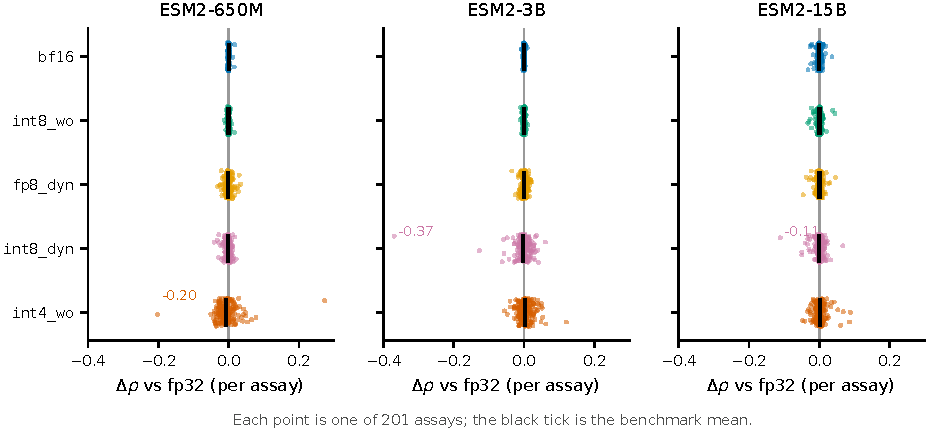
\includegraphics[width=\textwidth]{fig_tail.pdf}
\caption{Per-assay change in ground-truth correlation, all 201 assays, all three
scales. Black ticks are the benchmark mean, within $0.007$ of zero everywhere.
\cfg{bf16} and \cfg{int8\_wo} are tight at every assay and scale;
\cfg{int8\_dyn} and \cfg{int4\_wo} have equally unremarkable means and tails
reaching $-0.37$ and $-0.20$.}
\label{fig:tail}
\end{figure}

\begin{table}[htb]
\centering
\caption{Worst single-assay change in ground-truth correlation, with the count
of assays moving more than $0.05$ in parentheses, out of 201. The catastrophic
tail does not belong to a fixed configuration: \cfg{int4\_wo} at 650M,
\cfg{int8\_dyn} at 3B.}
\label{tab:tail3}
\small
\begin{tabular}{lrrr}
\toprule
Config & ESM2-650M & ESM2-3B & ESM2-15B \\
\midrule
\cfg{bf16}      & $-0.0040$ (0) & $-0.0072$ (0) & $-0.0323$ (0) \\
\cfg{int8\_wo}  & $-0.0120$ (0) & $-0.0106$ (0) & $-0.0329$ (0) \\
\cfg{fp8\_dyn}  & $-0.0316$ (0) & $-0.0344$ (0) & $-0.0465$ (0) \\
\cfg{int8\_dyn} & $-0.0411$ (0) & $\mathbf{-0.3688}$ (6) & $-0.1112$ (3) \\
\cfg{int4\_wo}  & $\mathbf{-0.2024}$ (6) & $-0.0556$ (5) & $-0.0472$ (5) \\
\bottomrule
\end{tabular}
\end{table}

\cfg{int8\_dyn} at 3B is indistinguishable from fp32 on the benchmark mean
($\Delta = -0.0021$, $p = 0.34$) while destroying
\texttt{UBR5\_HUMAN\_Tsuboyama\_2023\_1I2T}, where correlation with experiment
falls from $0.591$ to $0.223$ at $\rho_{\text{fp32}} = 0.393$. A configuration
can pass the benchmark average and be unusable on the one protein a project
cares about. Knowing which configuration was dangerous at one scale also does
not tell you which will be dangerous at another.

\subsubsection{At 15B the safe configurations degrade and the aggressive one improves}

Scale does not move all configurations in the same direction, and the crossover
needs a third point to see (Figure~\ref{fig:scale}c, Table~\ref{tab:fid3}).
\cfg{bf16} and \cfg{int8\_wo} do not drift measurably from fp32 on \emph{any} of
the 402 assay/model pairs at 650M and 3B, then drift on 13 and 15 assays at 15B,
with worst-case rank correlation falling to $0.857$ and $0.855$. \cfg{int4\_wo}
moves the other way: 182 assays below $\rho_{\text{fp32}} = 0.99$ at 650M, 154 at
3B, 82 at 15B.

\begin{table}[htb]
\centering
\caption{Fidelity against fp32 by scale: assays with $\rho_{\text{fp32}} < 0.99$
(of 201), and the worst single-assay value. The configurations that are safe at
small scale acquire a tail at 15B; the most aggressive one loses its tail.
Medians stay above $0.99$ everywhere, so none of this shows in a summary
statistic.}
\label{tab:fid3}
\small
\begin{tabular}{lrrrrrr}
\toprule
& \multicolumn{3}{c}{assays with $\rho_{\text{fp32}}<0.99$} & \multicolumn{3}{c}{worst $\rho_{\text{fp32}}$} \\
\cmidrule(lr){2-4}\cmidrule(lr){5-7}
Config & 650M & 3B & 15B & 650M & 3B & 15B \\
\midrule
\cfg{bf16}      &   0 &   0 & 13 & 0.9974 & 0.9905 & 0.8569 \\
\cfg{int8\_wo}  &   0 &   0 & 15 & 0.9963 & 0.9968 & 0.8548 \\
\cfg{fp8\_dyn}  &  29 &  18 & 19 & 0.9556 & 0.9770 & 0.8389 \\
\cfg{int8\_dyn} &  25 & 108 & 31 & 0.8894 & 0.3930 & 0.7645 \\
\cfg{int4\_wo}  & 182 & 154 & 82 & 0.6707 & 0.8791 & 0.8505 \\
\bottomrule
\end{tabular}
\end{table}

A natural reading is that a larger model carries more redundancy, so removing
weight precision costs proportionally less, while its activation dynamic range
grows until bf16's exponent becomes the binding constraint. We cannot assert
that mechanism from this data --- it would need a per-layer error analysis and
an fp16-versus-bf16 comparison, neither of which we ran. What the data does
support is that \textbf{the identity of the risky configuration is not stable
across scale}, so clearing a configuration at one scale does not clear it at
another. The 15B \cfg{bf16} degradation is also not a long-sequence artifact:
Spearman correlation between assay length and $\rho_{\text{fp32}}$ is $-0.14$,
and the five worst assays span $L = 222$ to $861$.

\begin{table}[htb]
\centering
\caption{The single worst-affected assay, by configuration and scale. No assay
appears twice: identifying the vulnerable target at one scale does not identify
it at another.}
\label{tab:worst3}
\small
\begin{tabular}{llrr}
\toprule
Scale & Config & Worst assay & $\Delta\rho$ \\
\midrule
650M & \cfg{bf16}      & \texttt{AICDA\_HUMAN\_Gajula\_2014\_3cycles} ($L{=}198$) & $-0.0040$ \\
650M & \cfg{int8\_dyn} & \texttt{POLG\_PESV\_Tsuboyama\_2023\_2MXD} ($L{=}53$)    & $-0.0411$ \\
650M & \cfg{int4\_wo}  & \texttt{B2L11\_HUMAN\_Dutta\_2010} ($L{=}198$)           & $-0.2024$ \\
\addlinespace
3B   & \cfg{bf16}      & \texttt{ODP2\_GEOSE\_Tsuboyama\_2023\_1W4G} ($L{=}44$)   & $-0.0072$ \\
3B   & \cfg{int8\_dyn} & \texttt{UBR5\_HUMAN\_Tsuboyama\_2023\_1I2T} ($L{=}58$)   & $-0.3688$ \\
3B   & \cfg{int4\_wo}  & \texttt{R1AB\_SARS2\_Flynn\_2022} ($L{=}306$)            & $-0.0556$ \\
\addlinespace
15B  & \cfg{bf16}      & \texttt{I6TAH8\_I68A0\_Doud\_2015} ($L{=}498$)           & $-0.0323$ \\
15B  & \cfg{int8\_dyn} & \texttt{GFP\_AEQVI\_Sarkisyan\_2016} ($L{=}238$)         & $-0.1112$ \\
15B  & \cfg{int4\_wo}  & \texttt{MBD11\_ARATH\_Tsuboyama\_2023\_6ACV} ($L{=}66$)  & $-0.0472$ \\
\bottomrule
\end{tabular}
\end{table}

\subsubsection{Resource envelope at 15B}

\begin{table}[htb]
\centering
\caption{ESM2-15B footprint. Peak memory during masked-marginals scoring is
almost entirely weights: the spread across 201 assays spanning $L = 37$ to $934$
is under $3$\,GB for every configuration. Quantization therefore addresses
essentially all of the DMS memory cost at this scale, and fp32 alone rules out
an 80\,GB A100. Model load takes about six minutes per configuration from the
shared filesystem, which is why the driver loads once and scores all 201 assays.}
\label{tab:res15b}
\small
\begin{tabular}{lrrrr}
\toprule
Config & Weights (GB) & \multicolumn{3}{c}{Peak memory over 201 assays (GB)} \\
\cmidrule(lr){3-5}
       &              & min & median & max \\
\midrule
\cfg{fp32}      & 56.36 & 56.51 & 57.09 & 59.30 \\
\cfg{bf16}      & 28.18 & 28.27 & 28.57 & 29.69 \\
\cfg{int8\_wo}  & 14.14 & 14.39 & 14.53 & 15.64 \\
\cfg{fp8\_dyn}  & 14.12 & 14.22 & 14.57 & 15.91 \\
\cfg{int8\_dyn} & 14.12 & 14.51 & 14.90 & 16.06 \\
\cfg{int4\_wo}  &  7.53 &  7.62 &  7.91 &  9.03 \\
\bottomrule
\end{tabular}
\end{table}

\subsubsection{The configuration ranking is scale-dependent}

Section~\ref{sec:opposite} reports that the two workloads prefer opposite
configurations. That holds at 650M and 3B and stops holding at 15B.

\begin{table}[htb]
\centering
\caption{DMS scoring speed relative to \cfg{bf16} over the full benchmark,
under both aggregation conventions. \emph{Throughput} is total masked positions
over total seconds, and is the figure consistent with the wall-clock hours of
Table~\ref{tab:speedram3}; \emph{median} is the median of the 201 per-assay
rates, which weights a 40-position assay as heavily as a 900-position one.
\cfg{bf16} runs at $174.2$, $93.7$ and $29.4$ positions/s by throughput and
$347.7$, $200.6$ and $56.7$ by median. \cfg{fp8\_dyn} closes on \cfg{bf16} as
scale grows under both, reaching parity at 15B: its overhead is per-call while
useful work grows with hidden size, so by 15B the GEMMs are compute-bound even
in the narrow-batch DMS regime. That same per-call overhead is why the two
conventions separate for \cfg{fp8\_dyn} and for no other configuration --- a
fixed cost per forward pass is proportionally worst on the short assays the
median weights most heavily.}
\label{tab:scale}
\small
\begin{tabular}{lrrrrrr}
\toprule
& \multicolumn{2}{c}{ESM2-650M} & \multicolumn{2}{c}{ESM2-3B} & \multicolumn{2}{c}{ESM2-15B} \\
\cmidrule(lr){2-3}\cmidrule(lr){4-5}\cmidrule(lr){6-7}
Config & tput & median & tput & median & tput & median \\
\midrule
\cfg{int8\_wo}  & $0.81\times$ & $0.72\times$ & $0.79\times$ & $0.69\times$ & $0.79\times$ & $0.72\times$ \\
\cfg{fp8\_dyn}  & $0.50\times$ & $0.30\times$ & $0.71\times$ & $0.44\times$ & $\mathbf{1.01\times}$ & $\mathbf{0.97\times}$ \\
\cfg{int8\_dyn} & $0.13\times$ & $0.07\times$ & $0.18\times$ & $0.10\times$ & $0.24\times$ & $0.20\times$ \\
\cfg{int4\_wo}  & $0.17\times$ & $0.16\times$ & $0.10\times$ & $0.09\times$ & $0.07\times$ & $0.07\times$ \\
\bottomrule
\end{tabular}
\end{table}

At 15B, \cfg{fp8\_dyn} scores the benchmark in $0.381$ GPU-hours against bf16's
$0.385$, at peak memory $14.57$ against $28.57$\,GB, with no measurable accuracy
cost. It is simply the better choice, which it is not at either smaller scale.
The workload conflict is a small-model phenomenon and a recommendation derived
at 650M or 3B does not transfer upward.

\begin{figure}[htb]
\centering
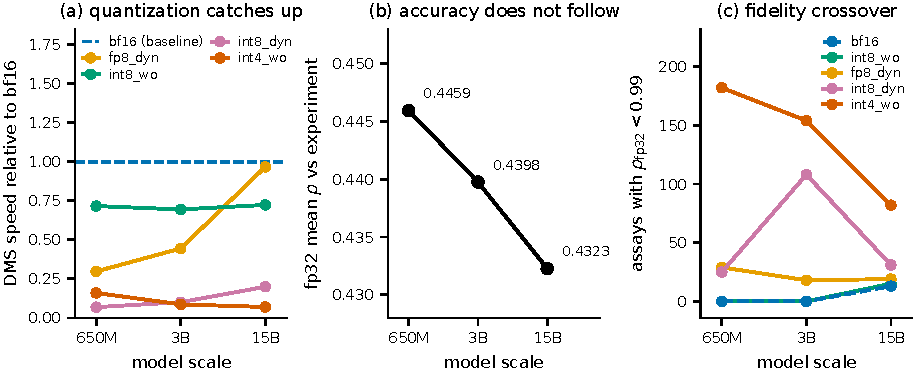
\includegraphics[width=\textwidth]{fig_scale.pdf}
\caption{Three effects visible only across scale. \textbf{(a)} DMS speed
relative to bf16, as aggregate throughput: \cfg{fp8\_dyn} converges on bf16
while the weight-only and INT4 paths do not. The dotted line repeats
\cfg{fp8\_dyn} under the median-of-assay convention --- the only configuration
for which the choice is visible, because its overhead is fixed per call and so
worst on the short assays a median weights most heavily. \textbf{(b)} fp32 mean Spearman falls monotonically across a
23-fold parameter increase; no pairwise difference is significant, but there is
no evidence that scale buys variant-effect accuracy. \textbf{(c)} Number of
assays where a configuration drifts from fp32 ($\rho_{\text{fp32}}<0.99$):
\cfg{bf16} and \cfg{int8\_wo} acquire a tail only at 15B while \cfg{int4\_wo}
sheds one.}
\label{fig:scale}
\end{figure}

\subsubsection{What the larger sample changed}

\textbf{The three-assay verdict was backwards, and the correction does not
resolve into a trend.} Section~\ref{sec:gt} concluded that quantization does not
systematically degrade variant-effect accuracy, on the evidence that 11 of 15
shifts were upward and \cfg{int4\_wo} gained $+0.0495$ on BLAT. At benchmark
scale \cfg{int4\_wo} is significantly harmful at 650M, significantly beneficial
at 3B, and null at 15B. Two scales would have left this looking like a trend in
model size; the third removes that reading.

\textbf{Fidelity predicts magnitude, not direction.} Across 3015
assay/configuration pairs, $r(1-\rho_{\text{fp32}},|\Delta|)$ is $0.74$, $0.81$
and $0.56$ at 650M, 3B, 15B. The $0.87$ first estimated from 15 pairs sits
above all three: the bound survives at scale, but weaker than the pilot
implied. The \emph{signed} correlation is $+0.10$, $-0.58$, $-0.40$: it does
not hold its sign across scales and is useless for prediction.

\begin{figure}[htb]
\centering
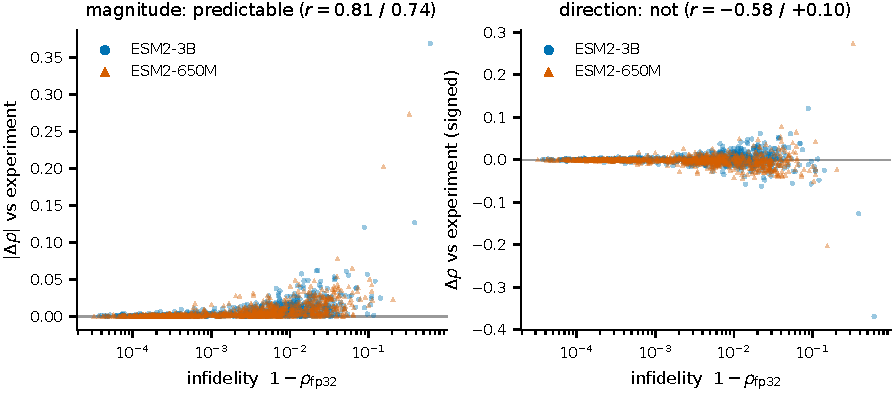
\includegraphics[width=\textwidth]{fig_fidelity.pdf}
\caption{Drift from fp32 against change in ground-truth correlation, 1005 pairs
per scale. \emph{Left:} infidelity bounds the magnitude of the change.
\emph{Right:} signed, the distribution is a symmetric funnel rather than a
trend, and the correlation changes sign between scales.}
\label{fig:fidelity}
\end{figure}

\textbf{Stratified effects do not replicate either.} At 650M, \cfg{int4\_wo}'s
cost is monotone in MSA depth ($-0.0174$, $-0.0050$, $-0.0042$ for low, medium,
high), inviting the reading that quantization harms most where the model has
least evolutionary signal. That ordering holds at 3B ($-0.0011$, $+0.0007$,
$+0.0097$) and breaks at 15B ($+0.0011$, $-0.0009$, $+0.0033$), where every
effect is inside the noise band anyway. Two scales agreeing and a third not is
exactly the pattern the \cfg{int4\_wo} result should teach us to distrust.

\subsubsection{The W8A8 collapse is a scaling defect, not a limit of the scheme}
\label{sec:w8a8fix}

``\cfg{int8\_dyn} destroys an assay'' and ``W8A8 cannot work for ESM-2'' carry
very different recommendations, so we tested which one the data supports.

Coarse granularity is not available as an explanation: \cfg{int8\_dyn} already
uses per-token activation and per-channel weight scales. We profiled
per-channel activation magnitudes at every encoder Linear input on the
collapsing assay and four length-matched controls, and \textbf{found no
distinguishing signature} --- outlier ratio median 16.8 against controls
15.5--17.2, and a largest raw activation of 14.8 against controls 14.9--17.5,
i.e.\ smaller. That negative result is about the diagnostic as much as the
mechanism: aggregating over 180 Linears washes out a defect localised to a few.

The intervention test is decisive where the diagnostic was not.

\begin{table}[htb]
\centering
\caption{Repairing W8A8 at 3B over the full benchmark. \cfg{int8\_dyn\_asym} is
the same config with asymmetric rather than symmetric activation quantization
--- one keyword, no calibration. \cfg{int8\_dyn\_sq} adds SmoothQuant
($\alpha = 0.5$, 16 calibration sequences). Both eliminate all six damaged
assays.}
\label{tab:w8a8}
\small
\begin{tabular}{lrrrrrr}
\toprule
Config & mean $\Delta$ & worst $\Delta$ & $|\Delta|>0.05$ & worst $\rho_{\text{fp32}}$ & pos/s & peak GB \\
\midrule
\cfg{int8\_dyn}       & $-0.0021$ & $\mathbf{-0.3688}$ & 6 & 0.393 & 17.0 & 3.51 \\
\cfg{int8\_dyn\_asym} & $-0.0001$ & $-0.0395$ & \textbf{0} & 0.965 & \textbf{33.1} & 4.13 \\
\cfg{int8\_dyn\_sq}   & $+0.0002$ & $\mathbf{-0.0237}$ & \textbf{0} & 0.737 & 16.9 & 3.66 \\
\bottomrule
\end{tabular}
\end{table}

\begin{figure}[htb]
\centering
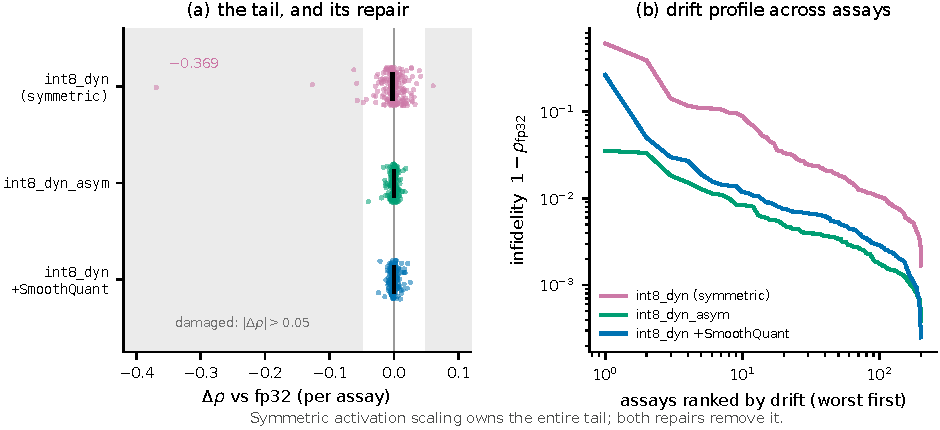
\includegraphics[width=\textwidth]{fig_w8a8.pdf}
\caption{\textbf{(a)} Per-assay $\Delta\rho$ for the three W8A8 variants;
shaded bands mark $|\Delta\rho|>0.05$, black ticks the mean. Symmetric scaling
owns the entire tail and both repairs remove it while the mean barely moves.
\textbf{(b)} Drift from fp32, assays ranked worst-first: the separation is not
confined to the tail --- symmetric is roughly threefold worse at the median.}
\label{fig:w8a8}
\end{figure}

\begin{figure}[htb]
\centering
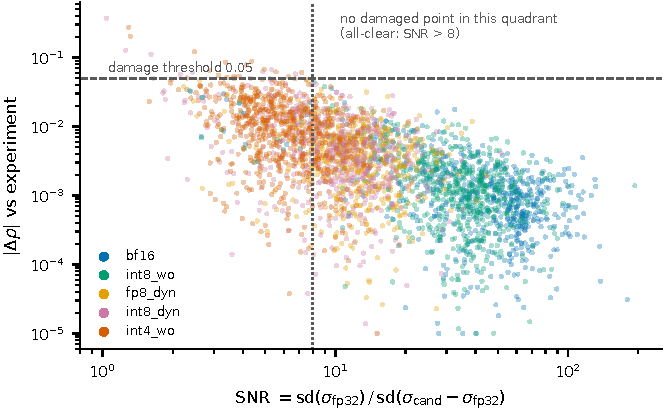
\includegraphics[width=0.72\textwidth]{fig_snr.pdf}
\caption{Signal-to-perturbation ratio against realised damage, 3015
combinations. The upper-right quadrant is empty: nothing above $\mathrm{SNR}=8$
loses more than $0.05$. Colour is the configuration, and their left-to-right
ordering recovers their aggressiveness unprompted.}
\label{fig:snr}
\end{figure}

Asymmetric scaling is the better remedy: no calibration, no prototype
dependency, and $1.95\times$ faster than symmetric \cfg{int8\_dyn} in our
measurements (20.6 against 40.0 minutes) at $0.6$\,GB more peak memory. We did
not investigate the speed difference. SmoothQuant reaches a slightly better
worst case ($-0.024$ against $-0.040$) but costs a calibration pass and has
\emph{poorer} worst-assay fidelity ($0.737$ against $0.965$).

So ``avoid \cfg{int8\_dyn}'' was too general. Its default \emph{symmetric}
activation scaling is unsafe on ESM-2 and a one-line change repairs it.

\subsubsection{A label-free screen for which assays are at risk}
\label{sec:snr}

What decides whether a ranking survives a perturbation is the perturbation
relative to the spread of the scores being perturbed. Both are computable
against fp32 on a user's own target, with no experimental labels:
$\mathrm{SNR} = \mathrm{sd}(\sigma_{\text{fp32}}) /
\mathrm{sd}(\sigma_{\text{cand}} - \sigma_{\text{fp32}})$.

\begin{table}[htb]
\centering
\caption{SNR against realised damage over all 3015 assay/configuration/scale
combinations. Every collapse beyond $0.10$ has $\mathrm{SNR} < 1.7$; nothing
with $\mathrm{SNR} > 8$ is damaged beyond $0.05$. Usable as an all-clear, not
as a precise predictor.}
\label{tab:snr}
\small
\begin{tabular}{lrrrr}
\toprule
SNR & $n$ & median $|\Delta|$ & $P(|\Delta| > 0.05)$ & worst $\Delta$ \\
\midrule
$< 2$    &   13 & 0.0478 & 46.2\% & $-0.3688$ \\
$2$--$4$ &  139 & 0.0165 &  7.2\% & $-0.0569$ \\
$4$--$8$ &  630 & 0.0092 &  1.4\% & $-0.0622$ \\
$> 8$    & 2233 & 0.0019 &  \textbf{0.0\%} & $-0.0409$ \\
\bottomrule
\end{tabular}
\end{table}

SNR is not merely re-discovering the configuration ranking. Median SNR runs from
$47.9$ (\cfg{bf16}) to $5.7$ (\cfg{int4\_wo}), but holding the configuration
fixed it still predicts damage within it --- Spearman $-0.43$, $-0.40$, $-0.26$,
$-0.39$, $-0.39$ for \cfg{bf16}, \cfg{int8\_wo}, \cfg{fp8\_dyn},
\cfg{int8\_dyn}, \cfg{int4\_wo}. Within \cfg{int4\_wo} alone the probability of
losing more than $0.05$ falls $10.5\% \to 1.6\% \to 0.0\%$ across
$\mathrm{SNR} < 4$, $4$--$8$, $>8$. It carries per-target information.

Reproduce with \texttt{python src/analyze\_scales.py} (section 5) and
\texttt{src/diag\_outliers.py}.

\subsubsection{Quantization competes with using a smaller model, and loses}

Every comparison so far is within a scale. That is the wrong frame for a
practitioner, who is not obliged to run 3B at all. Placing all three scales on
one Pareto surface over (accuracy, peak memory, speed), \textbf{only three of
eighteen configurations are non-dominated, and all three are 650M}
(Figure~\ref{fig:dominance}, Table~\ref{tab:pareto}).

\begin{table}[htb]
\centering
\caption{Cross-scale Pareto surface, all eighteen scale/configuration
combinations, ordered by accuracy. An option is dominated if another is at least
as good on accuracy, peak memory \emph{and} speed and strictly better on one;
the dominator named is in every case itself on the frontier. Speed is aggregate
throughput, and the frontier is unchanged under the median-of-assay convention.
3B/\cfg{int4\_wo} --- the configuration our recommendations table previously
offered for minimum memory --- uses more memory than 650M/\cfg{bf16} while being
less accurate and $19\times$ slower.}
\label{tab:pareto}
\small
\begin{tabular}{llrrrl}
\toprule
Scale & Config & mean $\rho$ & peak GB & pos/s & Status \\
\midrule
650M & \cfg{bf16}      & 0.4460 &  1.33 & 174.2 & \textbf{frontier} \\
650M & \cfg{int8\_wo}  & 0.4457 &  0.73 & 140.6 & \textbf{frontier} \\
650M & \cfg{int4\_wo}  & 0.4395 &  0.60 &  29.1 & \textbf{frontier} \\
\addlinespace
650M & \cfg{fp32}      & 0.4459 &  2.70 &  49.7 & dominated by 650M/\cfg{bf16} \\
650M & \cfg{fp8\_dyn}  & 0.4452 &  0.75 &  87.0 & dominated by 650M/\cfg{int8\_wo} \\
650M & \cfg{int8\_dyn} & 0.4440 &  0.75 &  23.0 & dominated by 650M/\cfg{int8\_wo} \\
\addlinespace
3B   & \cfg{int4\_wo}  & 0.4435 &  1.82 &   9.2 & dominated by 650M/\cfg{bf16} \\
3B   & \cfg{fp8\_dyn}  & 0.4403 &  2.90 &  66.6 & dominated by 650M/\cfg{bf16} \\
3B   & \cfg{bf16}      & 0.4399 &  5.50 &  93.7 & dominated by 650M/\cfg{bf16} \\
3B   & \cfg{int8\_wo}  & 0.4399 &  2.87 &  74.0 & dominated by 650M/\cfg{bf16} \\
3B   & \cfg{fp32}      & 0.4398 & 11.10 &  15.1 & dominated by 650M/\cfg{bf16} \\
3B   & \cfg{int8\_dyn} & 0.4376 &  2.94 &  17.0 & dominated by 650M/\cfg{bf16} \\
\addlinespace
15B  & \cfg{int4\_wo}  & 0.4332 &  7.91 &   2.1 & dominated by 650M/\cfg{bf16} \\
15B  & \cfg{fp8\_dyn}  & 0.4325 & 14.57 &  29.7 & dominated by 650M/\cfg{bf16} \\
15B  & \cfg{int8\_wo}  & 0.4325 & 14.53 &  23.4 & dominated by 650M/\cfg{bf16} \\
15B  & \cfg{bf16}      & 0.4323 & 28.57 &  29.4 & dominated by 650M/\cfg{bf16} \\
15B  & \cfg{fp32}      & 0.4323 & 57.09 &   3.3 & dominated by 650M/\cfg{bf16} \\
15B  & \cfg{int8\_dyn} & 0.4322 & 14.90 &   7.1 & dominated by 650M/\cfg{bf16} \\
\bottomrule
\end{tabular}
\end{table}

\begin{figure}[htb]
\centering
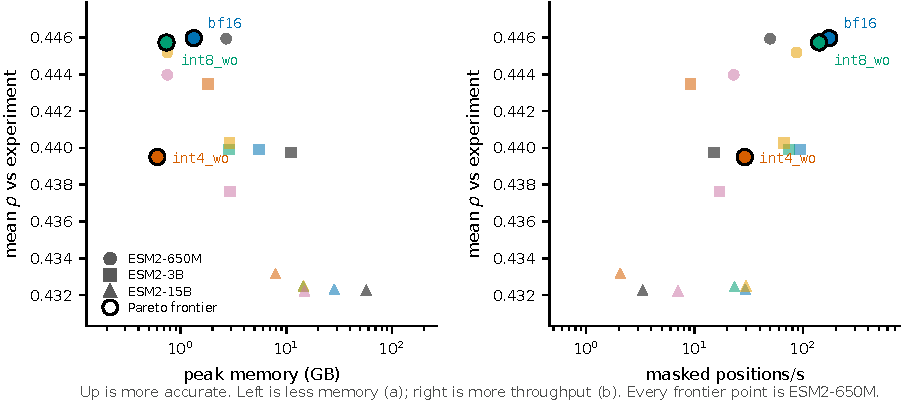
\includegraphics[width=\textwidth]{fig_dominance.pdf}
\caption{All eighteen scale/configuration combinations on two projections of the
Pareto surface. Higher is more accurate in both; the horizontal axes run in
opposite senses, so better is leftward against peak memory \textbf{(a)} and
rightward against throughput \textbf{(b)}. Circled points are non-dominated and
all are ESM2-650M.}
\label{fig:dominance}
\end{figure}

Quantization remains useful \emph{within} the frontier model:
650M/\cfg{int8\_wo} halves the memory of 650M/\cfg{bf16} for a $0.0002$ accuracy
change. But the memory-oriented configurations at 3B and 15B are not trade-offs
against a small model; they are strictly worse than one. This holds for
variant-effect scoring, where 650M is indistinguishable from 3B and 15B, and
does not transfer to tasks where the larger checkpoints are genuinely better.

\subsubsection{Interaction: is the effect actually different between scales?}

Calling \cfg{int4\_wo} ``significant in opposite directions'' rests on two
separate tests against fp32 whose verdicts are compared by eye, and those are
only nominally significant: 15 comparisons are reported (five configurations,
three scales) against a Bonferroni threshold of $0.0033$, and the two
\cfg{int4\_wo} results give $p = 0.0102$ and $p = 0.0104$.

The claim we want is that the effect \emph{differs} between scales, which is one
paired test on the same assays and is the stronger one.

\begin{table}[htb]
\centering
\caption{Interaction contrasts for \cfg{int4\_wo} at $R = 20{,}000$. The
3B--650M contrast survives Bonferroni correction for all 15 comparisons, where
neither individual test does. 15B does not differ from 3B, so the dependence is
not monotone.}
\label{tab:interaction}
\small
\begin{tabular}{lrlr}
\toprule
Contrast & Difference & 95\% CI & $p$ \\
\midrule
3B $-$ 650M  & $+0.0101$ & $[+0.0046,+0.0155]$ & $\mathbf{0.0007}$ \\
15B $-$ 650M & $+0.0073$ & $[+0.0021,+0.0123]$ & $0.0067$ \\
15B $-$ 3B   & $-0.0028$ & $[-0.0062,+0.0006]$ & $0.1017$ \\
\bottomrule
\end{tabular}
\end{table}

\subsubsection{Conditioning the tail on the reference having signal}

A large drop on an assay where fp32 itself scores near zero is rank instability,
not damage. Restricting to the 156--157 assays where fp32 reaches $\rho > 0.3$:
the 3B \cfg{int8\_dyn} collapse is unchanged at $-0.369$ (fp32 reaches $0.591$
there), while 650M \cfg{int4\_wo} falls from $-0.202$ to $-0.050$ and 15B
\cfg{int8\_dyn} from $-0.111$ to $-0.030$, because those occur where fp32
reaches only $0.270$ and $0.290$. Across cuts from $0.0$ to $0.4$ the 3B
\cfg{int8\_dyn} figure is invariant and the 650M \cfg{int4\_wo} figure is not,
so the central example is robust and the $-0.20$ figure is not.

On assays where the model is usable at all, \cfg{int8\_dyn} at 3B damages 2 of
157 and \cfg{int4\_wo} 4--5 of 157 by more than $0.05$ --- roughly a 1--3\%
chance a given target is affected.

\subsubsection{Speed and memory over the whole benchmark}

\begin{table}[htb]
\centering
\caption{Full 201-assay benchmark by scale, uncompiled, one H200. Wall-clock is
summed scoring time; peak memory is the median across assays. fp32 at 15B needs
57\,GB, so the reference configuration alone rules out an 80\,GB A100 once
activations are included.}
\label{tab:speedram3}
\small
\begin{tabular}{lrrrrrr}
\toprule
& \multicolumn{2}{c}{ESM2-650M} & \multicolumn{2}{c}{ESM2-3B} & \multicolumn{2}{c}{ESM2-15B} \\
\cmidrule(lr){2-3}\cmidrule(lr){4-5}\cmidrule(lr){6-7}
Config & hours & peak GB & hours & peak GB & hours & peak GB \\
\midrule
\cfg{fp32}      & 0.23 &  2.70 & 0.75 & 11.10 & 3.40 & 57.09 \\
\cfg{bf16}      & \textbf{0.07} &  1.33 & \textbf{0.12} &  5.50 & 0.39 & 28.57 \\
\cfg{int8\_wo}  & 0.08 &  0.73 & 0.15 &  2.87 & 0.48 & 14.53 \\
\cfg{fp8\_dyn}  & 0.13 &  0.75 & 0.17 &  2.90 & \textbf{0.38} & 14.57 \\
\cfg{int8\_dyn} & 0.49 &  0.75 & 0.67 &  2.94 & 1.61 & 14.90 \\
\cfg{int4\_wo}  & 0.39 &  \textbf{0.60} & 1.23 &  \textbf{1.82} & 5.47 &  \textbf{7.91} \\
\bottomrule
\end{tabular}
\end{table}

The DMS recommendation survives at 650M and 3B and inverts at 15B. Up to 3B,
\cfg{bf16} eager is fastest at every problem size --- $6.2\times$ faster than
fp32 end-to-end at 3B --- with ground-truth agreement never moving more than
$0.018$ across 402 assay/model pairs, and \cfg{int8\_wo} is the memory fallback
at roughly 80\% of bf16 throughput. At 15B, \cfg{fp8\_dyn} matches bf16 on speed at
half the memory and becomes the default. \cfg{int8\_dyn} and \cfg{int4\_wo} are
not trade-offs at any scale: slower than the best option \emph{and} owners of
the two worst tails in Table~\ref{tab:tail3}.

\section{Measurement Artifacts}

Four measurement defects were found and corrected during this study. Three of
them inverted or corrupted the very quantity being measured, and we document
them because each is a general hazard rather than a local mistake.

\subsection{Compile cost inside the timed region (three occurrences)}

The DMS throughput column initially ranked \cfg{fp32} fastest and \cfg{fp8\_dyn}
slowest --- an exact inversion of the bulk-throughput column. Two successive
fixes failed. Direct instrumentation finally established the cause. On
650M/A100 with a 40-residue wild type over 11 masked positions:

\begin{table}[htb]
\centering
\small
\begin{tabular}{lr}
\toprule
Measurement & Time \\
\midrule
eager, one forward at shape $(11, 42)$        & 27.9\,ms \\
eager, full \texttt{masked\_marginals} pass   & 0.03\,s \\
compiled, one forward at shape $(11, 42)$     & \best{15{,}138.1\,ms} \\
\bottomrule
\end{tabular}
\end{table}

DMS scoring uses a much smaller input shape than the bulk-throughput batches,
and under \texttt{max-autotune} each new shape costs roughly 15\,s to autotune.
At this batch size that cost recurs rather than amortizing. The timed region was
therefore measuring \emph{autotune cost}, and ranking configurations by their
number of Triton kernel candidates --- \cfg{fp32} had the fewest and appeared
fastest, \cfg{fp8\_dyn} had 98 and appeared slowest. The fix was to score DMS
against the uncompiled module.

This has a consequence beyond the benchmark: for short wild-type sequences with
few mutated positions, \texttt{max-autotune} is actively counterproductive in
production, not merely in measurement.

The same class of defect appeared earlier in the bulk-throughput path, where
warming up on only a prefix of the batches left recompilation for unseen length
buckets inside the timed region.

\subsection{Peak memory attributed to the wrong model}

Peak memory during DMS scoring was reported as follows, with the activation
overhead implied by subtracting weights:

\begin{table}[htb]
\centering
\small
\begin{tabular}{lrrr}
\toprule
Config & Weights (GB) & Peak (GB) & Implied overhead \\
\midrule
\cfg{fp32}      & 2.49 & 2.56 & $+0.07$ \\
\cfg{bf16}      & 1.21 & 3.74 & $+2.53 \approx$ fp32's weights \\
\cfg{int8\_wo}  & 0.61 & 1.86 & $+1.25 \approx$ bf16's weights \\
\cfg{int8\_dyn} & 0.61 & 1.26 & $+0.65 \approx$ int8\_wo's weights \\
\bottomrule
\end{tabular}
\end{table}

Each configuration's peak included the \emph{previous} configuration's weights,
producing the visible absurdity of bf16 requiring more peak memory than fp32.
The cleanup helper deleted only its own local reference to the model; the caller
retained a binding. Because \texttt{nn.Module} graphs contain reference cycles,
dropping the last reference does not free them by reference counting alone ---
they persist as cyclic garbage until a collection runs. Inserting an explicit
\texttt{gc.collect()} before each peak-memory reset corrected it; overhead
became a consistent 0.04--0.07\,GB.

The bulk-throughput memory column was verified unaffected: bf16's measured
overhead there was $+7.34$\,GB, which cannot contain fp32's 10.72\,GB of
weights.

\subsection{Silent argument leakage in the job script}

A batch script used \texttt{shift 3 || true}. When fewer than three positional
arguments are supplied, \texttt{shift 3} fails, \texttt{|| true} suppresses the
failure, and the arguments remain in \texttt{"\$@"} --- where they were appended
to the Python invocation as stray arguments. Relying on a default for the third
argument was sufficient to trigger it.

\subsection{Common thread}

Three of the four defects shared a signature: a cost that belonged outside the
measurement leaked inside it, and the resulting ranking was plausible enough to
be believed. In each case the tell was a result that inverted or contradicted a
neighbouring measurement. We would emphasise that a benchmark producing a
\emph{clean, monotonic, plausible} table is not thereby correct; the memory bug
produced exactly such a table for several runs.

\section{Discussion}

\subsection{The two workloads want opposite configurations}
\label{sec:opposite}

This is the principal practical finding.

\textbf{Bulk embedding extraction} is compute-bound: large batches, large GEMMs.
Quantization pays. \cfg{fp8\_dyn} with \texttt{max-autotune} wins on all three
axes --- $1.15\times$ bf16 throughput, weights $5.29 \to 2.65$\,GB, peak
$12.63 \to 7.24$\,GB, with accuracy indistinguishable from bf16.

\textbf{DMS variant-effect scoring} is latency-bound: the masked batch is small,
no GEMM is large enough for low precision to help, and per-linear
quantize/dequantize overhead is pure loss. bf16 in eager mode is fastest at
every problem size, and \texttt{max-autotune} is actively harmful.

Applying the embedding-optimized configuration to DMS scoring makes it up to an
order of magnitude slower. Because both workloads commonly appear in the same
pipeline, this is a live risk rather than a theoretical one.

\textbf{This conflict is bounded by scale, and one model could not have shown
that.} \cfg{fp8\_dyn}'s per-call quantization overhead is fixed while useful
work grows with hidden size, so the penalty shrinks as the model grows:
$0.50\times$ bf16 DMS throughput at 650M, $0.71\times$ at 3B, $1.01\times$ at 15B
(Table~\ref{tab:scale}). By 15B, \cfg{fp8\_dyn} is the right choice for
\emph{both} workloads at half the memory. The lesson is not that DMS is
latency-bound --- it is that whether a workload is latency-bound is a property
of the model and the workload together.

\subsection{On the interpretation of fidelity metrics}

The conventional validation practice --- quantize, measure drift against the
full-precision model, accept if drift is small --- is sound as a
\emph{risk bound}. Our data support the bound at scale: over 3015
assay/configuration pairs, fidelity loss correlates with the magnitude of
ground-truth change at $r = 0.74$, $0.81$ and $0.56$ at 650M, 3B and 15B,
--- the same relationship the 15-pair pilot found at $r = 0.87$, weaker at
every scale once the sample is large enough to resolve it.

It is not sound as a \emph{quality ranking}. A configuration with larger drift
is not thereby less accurate against reality; it is merely less predictable. The
signed correlation is $+0.10$, $-0.58$ and $-0.40$ at 650M, 3B and 15B --- it
does not hold its sign across model scales.

A tempting misreading of our BLAT result is that quantization acts as beneficial
regularization. We do not endorse this, and the full benchmark settles it:
\cfg{int4\_wo} is significantly \emph{negative} at 650M, significantly
\emph{positive} at 3B, and null at 15B. Two scales would have permitted the
reading that sensitivity falls with model size; the third removes it. A
configuration cannot be genuinely more accurate than the reference from which it
is derived in any way one could rely on in advance.

\subsection{Averages conceal the failure that matters}

The benchmark-mean result is that no configuration changes mean ground-truth
correlation by more than $0.007$. Read alone, that licenses any configuration on
the list. It should not.

\cfg{int8\_dyn} at 3B is statistically indistinguishable from fp32 on the mean
($p = 0.34$) and takes one assay from $\rho = 0.591$ to $0.223$. A practitioner
does not deploy against the mean of 201 assays; they deploy against one protein.
The benchmark mean answers whether a configuration is safe \emph{on average over
targets}, which is a claim about a population, while the operative question is
whether it is safe on a specific target.

The practical consequence is that the tail statistics --- worst-case single-assay
drift, and the count of assays exceeding a tolerance --- are the numbers to
select on, and they separate the configurations far more sharply than the means
do. On that criterion \cfg{bf16} and \cfg{int8\_wo} are safe (no assay beyond
$0.018$ across 402 assay/model pairs), \cfg{fp8\_dyn} is nearly so ($0.034$), and
\cfg{int8\_dyn} and \cfg{int4\_wo} are not.

\subsection{Recommendations}

\begin{table}[htb]
\centering
\small
\begin{tabular}{lll}
\toprule
Workload & Scale & Recommendation \\
\midrule
Bulk embedding extraction & any (H200)  & \cfg{fp8\_dyn} + \texttt{max-autotune-no-cudagraphs} \\
Bulk embedding extraction & any (A100)  & \cfg{int8\_dyn} \emph{asymmetric}; the symmetric \\
                          &             & \quad default is unsafe (Table~\ref{tab:w8a8}) \\
DMS / variant effect      & $\leq$ 3B   & \cfg{bf16}, eager, no compile \\
DMS / variant effect      & 15B         & \cfg{fp8\_dyn} --- matches bf16 speed at half the memory \\
DMS under memory pressure & $\leq$ 3B   & \cfg{int8\_wo} ($\sim$80\% of bf16 speed) \\
Minimum memory footprint  & any         & \cfg{int4\_wo}, only after confirming drift \\
                          &             & \quad on \emph{your} target; worst observed $-0.20$ \\
QLoRA fine-tuning base    & any         & \cfg{int4\_wo} \\
V100 / sm\_70 hardware    & any         & Quantization buys memory only, never speed \\
\bottomrule
\end{tabular}
\end{table}

Two non-quantization measures outweigh most of the above. Moving from fp32 to
bf16 is worth $8.4\times$ on bulk extraction and $6.2\times$ over the full DMS
benchmark; length-bucketed batching eliminates 25\% of wasted computation. Both
should be applied before any quantization is considered.

A third, proposed in an earlier draft of this report, does not survive the full
benchmark: the 650M checkpoint beat 3B by 0.14 Spearman on BLAT, which suggested
model selection dominated precision selection. Over 201 assays the two are
indistinguishable ($0.4459$ vs $0.4398$, 95\% CI $[-0.0061,+0.0185]$,
$p = 0.35$, with 650M ahead on 110 of 201). What remains true is narrower and
still useful: the \emph{uncertainty} on model choice ($\pm 0.012$) exceeds every
quantization effect measured here ($\leq 0.007$). Precision is the settled
variable; checkpoint choice is not, and is worth benchmarking on a
representative assay.

\section{Limitations}

\begin{itemize}
  \item \textbf{We still cannot predict which assays behave which way.} 201
        assays establish the population behaviour of each configuration and the
        size of its tail. They do not identify in advance which target will be
        the one that collapses. The only reliable procedure remains scoring a
        candidate configuration against fp32 on the actual target.
  \item \textbf{The 16 longest assays are excluded.} Assays beyond 1022
        residues exceed ESM-2's context and were skipped rather than truncated,
        since a truncation window is a scoring-protocol change that would
        confound the comparison. Configuration behaviour above $L = 934$ is
        therefore unmeasured.
  \item \textbf{Multiple comparisons are uncorrected.} Five configurations are
        tested against fp32 per model. Both significant results survive a
        Bonferroni threshold of $0.05/5 = 0.01$, but \cfg{int4\_wo} at 650M sits
        exactly on it ($p = 0.010$).
  \item \textbf{Bootstrap resolution.} Benchmark-level tests use $R = 20{,}000$
        and single-assay tests $R = 2000$; at 2000 resamples the smallest reportable
        two-sided $p$ is $0.001$; values at that floor should be read as
        $p < 0.002$ rather than as point estimates.
  \item \textbf{Low-signal assays resolve nothing individually.} Where
        $\rho_{\text{expt}} \approx 0.3$ the model's own error dominates and
        configuration differences fall below the noise floor; such assays
        contribute to the benchmark mean but carry little information alone.
  \item \textbf{Sequence-length coverage.} Bulk-throughput measurements used
        sequences of 512--1024 residues. Beyond $L \approx 2000$ the $O(L^2)$
        attention term dominates peak memory and quantization's share of the
        memory benefit shrinks correspondingly. A representative FASTA from the
        target workload would settle this.
  \item \textbf{Single random seed} for quantization; no ensemble over
        calibration variation.
  \item \textbf{The QLoRA track is unbuilt.} \cfg{int4\_wo} at 1.61\,GB is the
        natural base, and fine-tuning is the one setting where quantization buys
        capability rather than efficiency --- full 3B fine-tuning requires
        roughly 45\,GB of optimizer state alone.
\end{itemize}

\section{Conclusions}

\paragraph{What to run.} Two workloads, and the answer depends on model scale.

\begin{itemize}\setlength{\itemsep}{2pt}
  \item \textbf{Bulk embedding extraction: \cfg{fp8\_dyn} with
        \texttt{max-autotune}.} Best on all three axes at once at 3B ---
        $1.15\times$ bf16 throughput, peak memory $12.63 \to 7.24$\,GB, accuracy
        indistinguishable from bf16. Needs sm\_90; on A100, \cfg{int8\_wo}.
  \item \textbf{Variant-effect scoring up to 3B: \cfg{bf16}, eager,
        uncompiled.} Fastest at every problem size from $L=37$ to $934$,
        $6.2\times$ faster than fp32 over the full benchmark. Quantization is
        pure overhead and compilation is actively harmful.
  \item \textbf{Variant-effect scoring at 15B: \cfg{fp8\_dyn}.} Matches bf16
        throughput ($1.01\times$) at half the peak memory ($14.6$ vs $28.6$\,GB) with
        no measurable accuracy cost. The recommendation inverts with scale.
  \item \textbf{Avoid \cfg{int8\_dyn} and \cfg{int4\_wo} for variant-effect work
        at any scale.} Slower than the best option in this regime \emph{and}
        owners of the two worst tails measured, $-0.37$ and $-0.20$.
\end{itemize}

\paragraph{What the evidence says about evidence.}

\begin{enumerate}\setlength{\itemsep}{3pt}
  \item \textbf{Select on worst-case drift, not on benchmark means.} At no scale
        does any configuration move mean correlation by more than $0.007$ --- the
        statistic most likely to be quoted, and the one least able to
        distinguish these configurations. \cfg{int8\_dyn} passes the mean test at
        3B ($p = 0.34$) and takes one assay from $\rho = 0.591$ to $0.223$. On
        means, \cfg{int8\_dyn} and \cfg{bf16} differ by $0.002$; on worst case,
        by $0.36$ --- a factor of $180$.
  \item \textbf{Drift from fp32 is a valid safety certificate and an invalid
        quality ranking.} Over 3015 assay/configuration pairs it predicts the
        magnitude of ground-truth change ($r = 0.56$--$0.81$) and not its
        direction, whose correlation changes sign across model scales.
        \cfg{bf16} and \cfg{int8\_wo} never exceed $0.018$ Spearman on any of
        402 assay/model pairs up to 3B and are safe on that basis alone, which
        is cheap to verify on a target with no experimental labels.
  \item \textbf{Conclusions are bounded by model scale, not only by sample
        size.} The workload conflict holds at 650M and 3B and dissolves at 15B.
        The \cfg{int4\_wo} effect is significantly negative, significantly
        positive, then null in ascending scale order --- not a trend, so nothing
        to extrapolate. Even the MSA-depth stratification replicates at two
        scales and breaks at the third.
  \item \textbf{Evidence scale is not a matter of rigour but of conclusions.}
        This study reached four successive verdicts. A synthetic mutational scan
        ranked configurations confidently and wrongly. Three real assays
        overturned it and produced two further generalisations --- that
        quantization does not systematically degrade accuracy, and that
        checkpoint choice dominates precision choice --- both reversed by the
        full 201-assay benchmark. That benchmark at two scales then suggested
        sensitivity grows with model size, which the third scale removed. Every
        intermediate conclusion was statistically sound on its own data. The
        full three-scale benchmark costs 16.2 GPU-hours.
\end{enumerate}

\paragraph{The general claim.} A benchmark mean answers whether a configuration
is safe \emph{on average over targets}. Deployment asks whether it is safe on
\emph{one} target. Here those questions differ by the gap between $0.002$ and
$0.36$. Wherever a benchmark aggregates over heterogeneous instances and the
user faces one instance, we would report the tail alongside the mean as a matter
of course.

\section{Reproduction}

\begin{footnotesize}
\begin{verbatim}
# Environment (handles glibc/GCC/cache-quota constraints)
source env/activate.sh

# Fetch assay data; verifies variant indexing against target_seq
python src/fetch_proteingym.py IF1_ECOLI_Kelsic_2016 \
    BLAT_ECOLX_Stiffler_2015 HSP82_YEAST_Flynn_2019

# Bulk throughput + fidelity matrix (compiled)
sbatch -p H8V141_SAP112M2000_L --mem=200G slurm/run_matrix.sbatch \
    3B fp32,bf16,int8_wo,int8_dyn,fp8_dyn,int4_wo --compile

# Real-assay DMS: accuracy, speed, memory (uncompiled by design)
sbatch -p H8V141_SAP112M2000_L --mem=200G slurm/run_dms.sbatch \
    3B fp32,bf16,int8_wo,int8_dyn,fp8_dyn,int4_wo

# Significance of ground-truth shifts (single assay, variant bootstrap)
python src/analyze_dms.py results/dms_3B_*_<jobid>_scores.json

# --- Full benchmark ---------------------------------------------------
# All 217 assays; validates every variant's WT and refuses to write on
# mismatch.  ~110 MB of parquet, cached in data/proteingym_v1/_raw
python src/fetch_proteingym_v1.py

# One array task per config; each loads its model once and scores all
# 201 assays.  Resumable: a resubmission skips assays already written.
sbatch --array=0-5 -p H8V141_SAP112M2000_L --mem=200G \
    slurm/run_proteingym.sbatch 3B
sbatch --array=0-5 -p H8V141_SAP112M2000_L --mem=200G \
    slurm/run_proteingym.sbatch 650M
# 15B needs more memory and wall time (int4_wo alone is 5.5 h)
sbatch --array=0-5 -p H8V141_SAP112M2000_L --mem=300G --time=12:00:00 \
    slurm/run_proteingym.sbatch 15B

# The two W8A8 repairs: asymmetric activations, and SmoothQuant with
# 16 calibration sequences.
sbatch --array=0-1 -p H8V141_SAP112M2000_L --mem=200G \
    slurm/run_proteingym.sbatch 3B int8_dyn_asym,int8_dyn_sq

# Benchmark-wide accuracy / speed / RAM + protein-clustered bootstrap
python src/aggregate_proteingym.py --model 3B
python src/aggregate_proteingym.py --model 650M
python src/aggregate_proteingym.py --model 15B

# --- Analyses reported here -------------------------------------------
# Pareto surface, interaction contrasts, conditioned tail, aggregation
# conventions with post-stratification, and the SNR screen
python src/analyze_scales.py

# W8A8 repair, per assay -> results/proteingym/w8a8_remedies.csv
python src/analyze_w8a8.py

# Repeatability floor: rep2 against the primary run, bitwise
python src/analyze_repeat.py

# Per-channel activation profile of the collapsing assay vs controls
sbatch -p H8V141_SAP112M2000_L --mem=200G slurm/run_outliers.sbatch

# Figures (also used by the preprint)
python src/figures.py
\end{verbatim}
\end{footnotesize}

\noindent
Result artifacts referenced in this report:

\begin{footnotesize}
\begin{itemize}\setlength{\itemsep}{0pt}
  \item Throughput matrices (SLURM jobs 5393462, 5393520, 5393524, 5393554):\\
        \texttt{results/matrix\_3B\_<jobid>.json}
  \item ProteinGym, 3B, with per-variant scores (job 5394386):\\
        \texttt{results/dms\_3B\_<assay>\_5394386.json}
  \item ProteinGym, 650M (job 5394316):
        \texttt{results/dms\_650M\_<assay>\_5394316.json}
  \item Full benchmark, per-variant scores: 3B (array 5395036),
        650M (array 5395037), 15B (array 5395122):\\
        \texttt{results/proteingym/<model>\_<config>.jsonl.gz}
  \item Full-benchmark analysis:
        \texttt{results/proteingym/summary\_<model>.json} and\\
        \texttt{summary\_<model>\_per\_assay.csv} (1206 rows at 650M and
        15B, 1608 at 3B: one per
        assay/configuration)
\end{itemize}
\end{footnotesize}

\end{document}
